\documentclass[a4paper,11pt]{article}
\pdfoutput=1 % if your are submitting a pdflatex (i.e. if you have
             % images in pdf, png or jpg format)

\usepackage{jinstpub} % for details on the use of the package, please
                     % see the JINST-author-manual
\usepackage{lineno}
\usepackage{amsmath}

\linenumbers

\author{The MicroBooNE Collaboration}
\title{First Neutrino-Induced-Muon Momentum Determination by Multiple Coulomb Scattering in a LArTPC}


%% %simple case: 2 authors, same institution
%% \author{A. Uthor}
%% \author{and A. Nother Author}
%% \affiliation{Institution,\\Address, Country}

% % more complex case: 4 authors, 3 institutions, 2 footnotes
% \author[a,b,1]{F. Irst,\note{Corresponding author.}}
% \author[c]{S. Econd,}
% \author[a,2]{T. Hird\note{Also at Some University.}}
% \author[c,2]{and Fourth}

% % The "\note" macro will give a warning: "Ignoring empty anchor..."
% % you can safely ignore it.

% \affiliation[a]{One University,\\some-street, Country}
% \affiliation[b]{Another University,\\different-address, Country}
% \affiliation[c]{A School for Advanced Studies,\\some-location, Country}

% % e-mail addresses: only for the forresponding author
% \emailAdd{first@one.univ}


\abstract{Liquid Argon Time Projection Chambers (LArTPCs) are an important detector technology for the future of neutrino physics. This technology provides precise three-dimensional reconstruction of charged particle tracks that traverse the detector medium. 
%The MicroBooNE experiment is a LArTPC at the Fermi National Accelerator laboratory with active volume dimensions of 2.6 m width $\times$ 2.3 m height $\times$ 10.4 m length located in the Booster Neutrino Beamline (BNB) which has a peak neutrino energy of about 0.7 GeV. 
We discuss a technique for measuring a charged particle's momentum by means of multiple coulomb scattering (MCS) in the MicroBooNE LArTPC, which does not require the full particle ionization track to be contained inside of the detector volume as other track momentum reconstruction methods do (range-based momentum reconstruction and calorimetric momentum reconstruction). We provide motivation for why this technique is important, and quantify its performance on fully contained beam-neutrino-induced muon tracks both in simulation and in data. In general we find agreement between data and simulation, with small bias in the momentum reconstruction and with resolutions that vary as a function of track length, decreasing from about 12\% for the shortest (one meter long) tracks to nearly 5\% for longer (several meter) tracks.}


% \keywords{Only keywords from JINST's keywords list please}


% \arxivnumber{1234.56789} % only if you have one


% \collaboration{\includegraphics[height=17mm]{example-image}\\[6pt]
%   XXX collaboration}
% or
% \collaboration[c]{on behalf of XXX collaboration}


% if you write for a special issue this may be useful
% \proceeding{N$^{\text{th}}$ Workshop on X\\
%   when\\
%   where}



\begin{document}
\maketitle
\flushbottom

\section{Introduction and Motivation}\label{sec:intro}

MicroBooNE (Micro Booster Neutrino Experiment) is an experiment based at the Fermi National Accelerator Laboratory (Fermilab) that uses a large Liquid Argon Time Projection Chamber (LArTPC) to investigate the excess of low energy events observed by the MiniBooNE experiment \cite{Aguilar-Arevalo:2013pmq} and to study neutrino-argon cross-sections. MicroBooNE is part of the Short-Baseline Neutrino (SBN) physics program, along with two other LArTPCs: the Short Baseline Near Detector (SBND) and the Imaging Cosmic And Rare Underground Signal (ICARUS) detector. MicroBooNE also provides important research and development in terms of detector technology and event reconstruction techniques for future LArTPC experiments including DUNE (Deep Underground Neutrino Experiment).\\

\begin{figure}[ht!]
\centering
	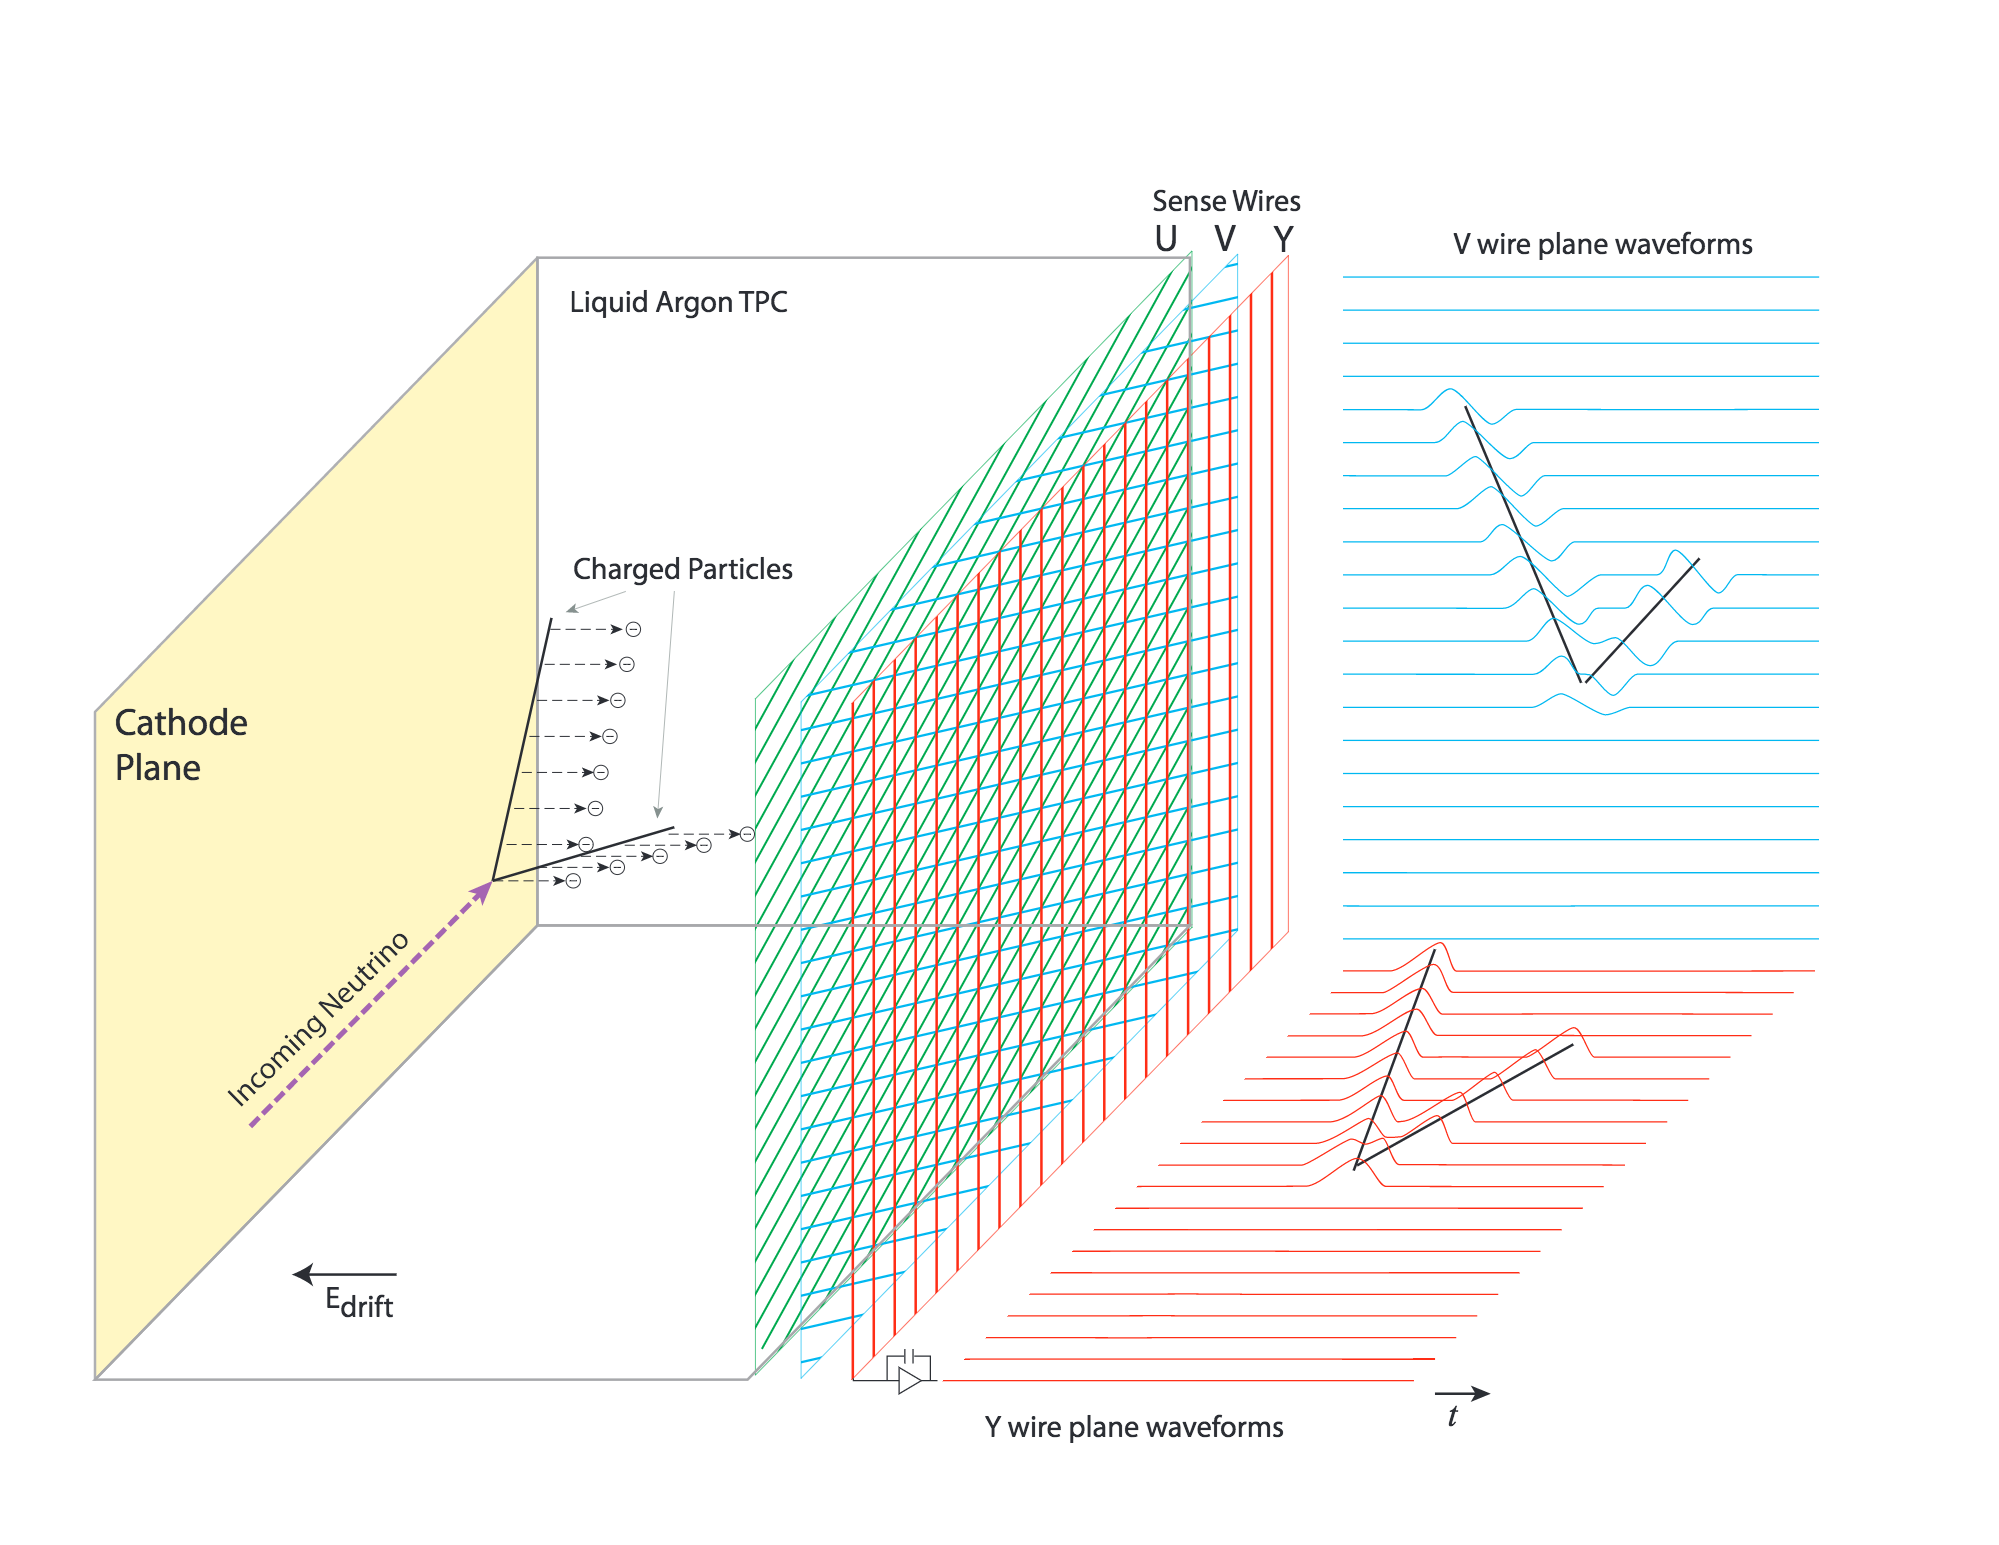
\includegraphics[width=0.9\textwidth]{Figures/static_figs/detector2.png} \\
\caption{\textit{A diagram of the time projection chamber of the MicroBooNE detector \cite{lartpc}.}}\label{detector_fig}
\end{figure}

The MicroBooNE detector\cite{ub_detectorpaper} consists of a rectangular time projection chamber (TPC) with dimensions 2.6 m width $\times$ 2.3 m height $\times$ 10.4 m length located 470 m away from the Booster Neutrino Beam (BNB) target. LArTPCs allow for precise three-dimensional reconstruction of particle interactions. The $x-$ direction of the TPC corresponds to the drift coordinate, the $y-$ direction is the vertical direction, and the $z-$ direction is the direction along the beam. The mass of active liquid argon in the MicroBooNE TPC is 89 tons, with the total cryostat containing 170 tons of liquid argon.\\

A set of 32 photomultiplier tubes (PMTs) and three wire planes with 3 mm spacing at angles of 0, and $\pm$ 60 degrees with respect to the vertical are located in the TPC for event reconstruction (Figure \ref{detector_fig}). In a neutrino interaction, a neutrino from the beam interacts with an argon nucleus and the charged outgoing secondary particles traverse the medium, losing energy and leaving an ionization trail. The resulting ionization electrons drift to the anode side of the TPC, containing the wire planes. The passage of these electrons near the first two wire planes induces a signal in them and their collection on the third plane also generates a signal. These signals are used to create three distinct two-dimensional views (in terms of wire and time) of the event. Combining these wire signals with timing information from the PMTs allows for full three-dimensional reconstruction of the event.\\

The Booster Neutrino Beam (BNB) is predominantly composed of muon neutrinos ($\nu_\mu$) with a peak neutrino energy of about 0.7 GeV, which can undergo charge-current ($\nu_\mu$CC) interactions in the TPC and produce muons. For muon tracks that are completely contained in the TPC, it is straightforward to calculate their momentum with a measurement of the length of the particle's track, or with calorimetric measurements which come from wire signal measurements. However, around half of muons from BNB neutrino events in MicroBooNE are not fully contained in the TPC, and therefore using length-based calculations for these uncontained tracks is not a possibility. The only way to compute the energy of a non-contained three-dimensional track is by means of multiple coulomb scattering (MCS). \\

Multiple Coulomb Scattering (MCS) occurs when a charged particle enters a medium and undergoes electromagnetic scattering with the atomic nuclei. This scattering deviates the original trajectory of the particle within the material (Figure \ref{mcs_nocap_fig}). For a given energy, the angular deflection scatters of a particle in either the $x'$ direction or $y'$ direction (as indicated in the aforementioned figure) form a gaussian distribution centered at zero with a width, $\sigma_o^{HL}$ given by the Highland formula \cite{highland}: 

\begin{equation}\label{highland_eqtn}
	\sigma_o^{HL}=\frac{13.6\  \text{MeV}}{p\beta c}z\sqrt{\frac{\ell}{X_0}}\Big[1+0.0038\text{ln}\Big(\frac{\ell}{X_0}\Big)\Big]
\end{equation}

\noindent where $\beta$ is the ratio of the particle's velocity to the speed of light, $\ell$ is the distance traveled inside the material, $z$ is the magnitude of the charge of the particle, and $X_0$ is the radiation length of the target material (taken to be a constant 14 cm in liquid argon). In practice, a modified version of the Highland formula is used
\begin{equation}\label{modified_highland_eqtn}
\sigma_{o} = \sqrt{ (\sigma_o^{HL})^2 + (\sigma_o^{res})^2} = \sqrt{ (\frac{13.6\  \text{MeV}}{p\beta c}z\sqrt{\frac{\ell}{X_0}}\Big[1+0.0038\text{ln}\Big(\frac{\ell}{X_0}\Big)\Big])^2 + (\sigma_o^{res})^2 }
\end{equation}
where the formula is ``modified'' from the original Highland formula (Equation \ref{highland_eqtn}) in that it includes a detector-inherent angular resolution term, $\sigma_o^{res}$. For this analysis, this term is given a fixed value of 2 mrad which has been determined to be an acceptable value based on simulation studies.\\


With the Highland formula, the momentum of a track-like particle can be determined using only the 3D reconstructed track it produces in the detector, without any calorimetric or track range information. The method by which this is done is described in detail in Section \ref{MCS_technique_section} and was originally described for use in a LArTPC on atmospheric muons by the ICARUS collaboration\cite{icarus_mcs_paper}.

\begin{figure}[ht!]
\centering
	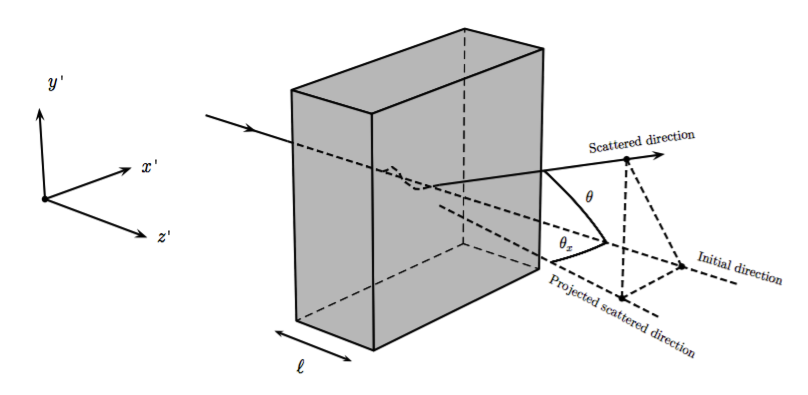
\includegraphics[width=0.9\textwidth]{Figures/static_figs/mcs_nocap.png} \\
\caption{\textit{The particle's trajectory is deflected as it traverses through the material.}}\label{mcs_nocap_fig}
\end{figure}

























\section{MCS Implementation Using the Maximum Likelihood Method}\label{MCS_technique_section}

This section describes exactly how the phenomenon of multiple coulomb scattering is leveraged to determine the momentum of a track-like particle reconstructed in a LArTPC. In general, the approach is as follows:
\begin{enumerate}
\item The three-dimensional track is divided into segments of configurable length.
\item The scattering angles between consecutive segments are measured.
\item Those angles combined with the modified Highland formula (Equation \ref{modified_highland_eqtn}) are used to build a likelihood that the particle has a specific momentum, taking into account energy loss in upstream segments of the track.
\item The momentum corresponding to the maximum likelihood is chosen to be the MCS computed momentum.
\end{enumerate}
Each of these steps are discussed in detail in the following subsections.\\

% For this analysis, a minimum start-to-end reconstructed track length of 100 cm was used. A minimum length is required to allow for sufficient scatters to measure the momentum. With 100 cm tracks and 10 cm segments (see Section \ref{track_segmentation_section}), twenty scattering measurements will ultimately be used to reconstruct the momentum of the particle (see Section \ref{scattering_angle_computation_section}).













\subsection{Track Segmentation and Scattering Angle Computation}\label{track_segmentation_and_scattering_angle_computation_section}
% The input to the track segmentation routine is a vector of ordered three-dimensional trajectory points (x,y,z) representing the reconstructed track. The points are ordered along the direction of the track, with the first point representing the start of the track, and the last point representing the end of the track. These trajectory points can be determined in a number of ways by different track reconstruction algorithms. In the case of this analysis, the track reconstruction algorithm is named ``pandoraNuPMA" which constructs these three-dimensional trajectory points by combining two-dimensional hits reconstructed from signals on the different wire planes along with timing information from the photomultiplier tubes to reconstruct the third dimension\cite{Marshall:2015rfa}. Note that the tracking resolution in the y- (vertical) and z- (beam) directions are determined by the wire plane spacings, while the resolution in the x- (drift) direction is determined by optical signal timing and is therefore the x- direction resolution is better than that of the y- and z- directions.\\

% Also input to the track segmentation routine is the desired segment length, which is a tunable parameter. In this note, segment lengths are always taken to be 10 cm (based on the findings of Appendix \ref{SegmentLength_MCBNBRecoTrack_section}) except where otherwise explicitly stated. 
Track segmentation refers to the subdivision of three-dimensional reconstructed trajectory points of a reconstructed track into portions of definite length. In this analysis, the tracks are automatically reconstructed by the ``pandoraNuPMA" projection matching algorithm which constructs the three-dimensional trajectory points by combining two-dimensional hits reconstructed from signals on the different wire planes along with timing information from the photomultiplier tubes to reconstruct the third dimension\cite{Marshall:2015rfa}. The segmentation routine begins at the start of the track, and iterates through the trajectory points in order, defining segment start and stop points based on the straight-line distance between them. There is no overlap between segments. Given the subset of the three-dimensional trajectory points that correspond to one segment of the track, a three-dimensional linear fit is applied to the data points, weighing all trajectory points equally in the fit. In this analysis, a segment length of 10 cm is used, which is a tunable parameter that has been optimized based on simulation studies.\\

With the segments defined, the scattering angles between adjacent segments are computed. A coordinate transformation is performed such that the $z'$ direction is oriented along the direction of the first of the segment pair. The $x'$ and $y'$ coordinates are then defined such that all of $x'$, $y'$, and $z'$ are mutually orthogonal, as shown in Figure \ref{mcs_nocap_fig}. The scattering angles both with respect to the $x'$ direction and the $y'$ direction are then computed to be used by the MCS algorithm. Note that only the scattering angle with respect to the $x'$ direction is drawn in Figure \ref{mcs_nocap_fig}.



% This routine within the MCS code takes as input the vector of length $n$ (where $n$ is the number of segments for the track) containing the direction cosines at the start of each segment. In general, the algorithm iterates over consecutive pairs of segments (the segmentation routine is described in Section \ref{track_segmentation_section}) and computes angular scatters between each, and stores them for later use by a future subroutine. This code is more complicated than just taking the dot product between consecutive direction cosines to find the total angular scatter between segments because the Highland formula is derived from scattering independently in the two directions orthogonal to the direction of the track. For this reason, this subroutine performs a coordinate transformation for each pair of segments such that the direction of first of the two segments is along the $z'$ direction, as drawn in Figure \ref{mcs_nocap_fig}. With the $z'$ direction defined as such, $x'$ and $y'$ directions are chosen such that all of $x'$, $y'$, and $z'$ are mutually orthogonal, again shown in Figure \ref{mcs_nocap_fig}\footnote{Note that at this point, all of $x'$, $y'$, and $z'$ are different than the detector coordinates, $x$, $y$, and $z$ which correspond to drift direction, vertical direction, and beam direction respectively.}. The scattering angles both in the $x'$ and $y'$ planes are then computed for each consecutive pairs of segments\footnote{Both of these scattering angles are used downstream in the MCS algorithm, and therefore the choice of $x'$ and $y'$ are not important.}. After this routine, a vector of length $2n$ is stored containing the scattering angles in the $x'$ plane as well as in the $y'$ plane. These scattering angles are what are input into the maximum likelihood routine to determine track momentum.














\subsection{Maximum Likelihood Theory}\label{likelihood_theory_section}

The normal probability distribution for the scattering angle in either the $x'$ or $y'$ direction, $\Delta\theta$ with an expected gaussian error $\sigma_o$ and mean of zero is given by:
\begin{equation}
f_X(\Delta\theta) = (2\pi\sigma_o^2)^{-\frac{1}{2}}exp(-\frac{1}{2}(\frac{\Delta\theta}{\sigma_o})^2)
\end{equation}

Here, $\sigma_o$ is the RMS angular deflection computed by the modified Highland formula (Equation \ref{modified_highland_eqtn}), which is a function of both the momentum and the length of that segment. Since energy is lost between segments along the track, $\sigma_o$ increases for each angular measurement along the track so we replace $\sigma_o$ with $\sigma_{o,j}$, where $j$ is an index representative of the segment. \newline

To get the likelihood, one takes the product of $f_X(\Delta\theta_j)$ over all $n$ of the $\Delta\theta_j$ segment-to-segment scatters along the track. With some manipulation, this product becomes
\begin{equation}
L((\sigma_{o,1})^2,...,(\sigma_{o,n})^2;\Delta\theta_1,...,\Delta\theta_n) = (2\pi)^\frac{-n}{2}\times\prod_{j=1}^{n}(\sigma_{o,j})^{-1} \times exp(-\frac{1}{2}\sum_{j=1}^{n}(\frac{\Delta\theta_j}{\sigma_{o,j}})^2)
\end{equation}

In practice, rather than maximizing likelihood it is often more computationally convenient to instead minimize the negative log likelihood. Inverting the sign and taking the natural logarithm of the likelihood $L$ gives an expression that is related to a $\chi^2$
\begin{equation}\label{leo_llhd_eqtn}
-l(\mu_o;(\sigma_{o,1})^2,...,(\sigma_{o,n})^2;\Delta\theta_1,...,\Delta\theta_n) = -ln(L) = \frac{n}{2}ln(2\pi) + \sum_{j=1}^{n}ln(\sigma_{o,j}) + \frac{1}{2}\sum_{j=1}^{n}(\frac{\Delta\theta_j}{\sigma_{o,j}})^2
\end{equation}

% The negative log likelihood for one specific segment's angular scatter $\Delta\theta_j$ given an expected scattering RMS $\sigma_{o,j}$ is given by the following equation
% \begin{equation}\label{negative_llh_eqtn}
% -l(\mu_o, \sigma_{o,j}, \Delta\theta_j) = \frac{1}{2}ln(2\pi) + ln(\sigma_{o,j}) + \frac{1}{2}\frac{(\Delta\theta_j-\mu_o)^2}{(\sigma_{o,j})^2}
% \end{equation}

% In general, Equation \ref{negative_llh_eqtn} is evaluated for each segment in a track given a postulated full track momentum, and the sum of these terms is used to determine the likelihood that the postulated track momentum is correct for that track.











\subsection{Maximum Likelihood Implementation}\label{maximum_likelihood_section}

Given a set of angular deflections in the $x'$ and $y'$ directions for each segment as described in Section \ref{track_segmentation_and_scattering_angle_computation_section} a raster scan over postulated track momenta in steps of 1 MeV up to 7.5 GeV is computed and the step with the smallest negative log likelihood (Equation \ref{leo_llhd_eqtn}) is chosen as the final MCS momentum. Note that Equation \ref{leo_llhd_eqtn} includes a $\sigma_{o,j}$ term which changes for each consecutive segment because their energies are decreasing. The energy of the $j$th segment is given by

\begin{equation}\label{segment_E_equation}
E_{j} = E_t - k_{cal}*N_{upstream}*l_{seg}
\end{equation}

where $k_{cal}$ is the minimally ionizing energy constant taken to be $2.105 \frac{MeV}{cm}$ in liquid argon\cite{MIPenergysource}, $N_{upstream}$ is the number of segments upstream of the $j$th segment, and $l_{seg}$ is the 3D segment length. This definition of $E_j$ therefore takes into account energy loss along the track. Note that Equation \ref{segment_E_equation} introduces a minimum allowable track energy determined by the length of the track, as $E_{j}$ must remain positive. This value of segment energy is converted to a momentum, $p$, with the usual energy-momentum relation, assuming the muon mass, and is then used to predict the RMS angular scatter for that segment ($\sigma_o$) by way of Equation \ref{modified_highland_eqtn}. 



















\section{Range-based Energy Validation from Simulation}\label{Range_Energy_Validation_section}
In order to quantify the performance of the MCS energy estimation method on fully contained muons in data, an additional handle on energy is needed. Here, range-based energy is used. The stopping power of muons in liquid argon is well described by the particle data group (PDG)\cite{PDG_spline_table}. By using a linear interpolation between points in the cited PDG stopping power table, the start-to-end straight-line length of a track can be used to reconstruct the muon's total energy with good accuracy. A simulated sample of fully contained BNB neutrino-induced muons longer than one meter is used to quantify the bias and resolution for the range-based energy estimation technique. The range is defined as the straight-line distance between the true starting point and true stopping point of a muon. The bias and resolution are computed in bins of true total energy of the muons by fitting a gaussian to a distribution of the fractional energy difference ($\frac{E_{Range}-E_{True}}{E_{True}}$) in each bin. The mean of each gaussian indicates the bias for that true energy bin, and the width indicates the resolution. Figure \ref{true_range_bias_resolution_MCTrack_fig} shows the bias and resolution for the range-based energy reconstruction method. It can be seen that the bias is negligible and the resolution for this method of energy reconstruction is on the order of 2-4\%. Based on this figure, it is clear that range-based energy (and therefore range-based momentum) is a good handle on the true energy (momentum) of a reconstructed muon track in data, assuming that the track is well reconstructed in terms of length.

\begin{figure}
\centering
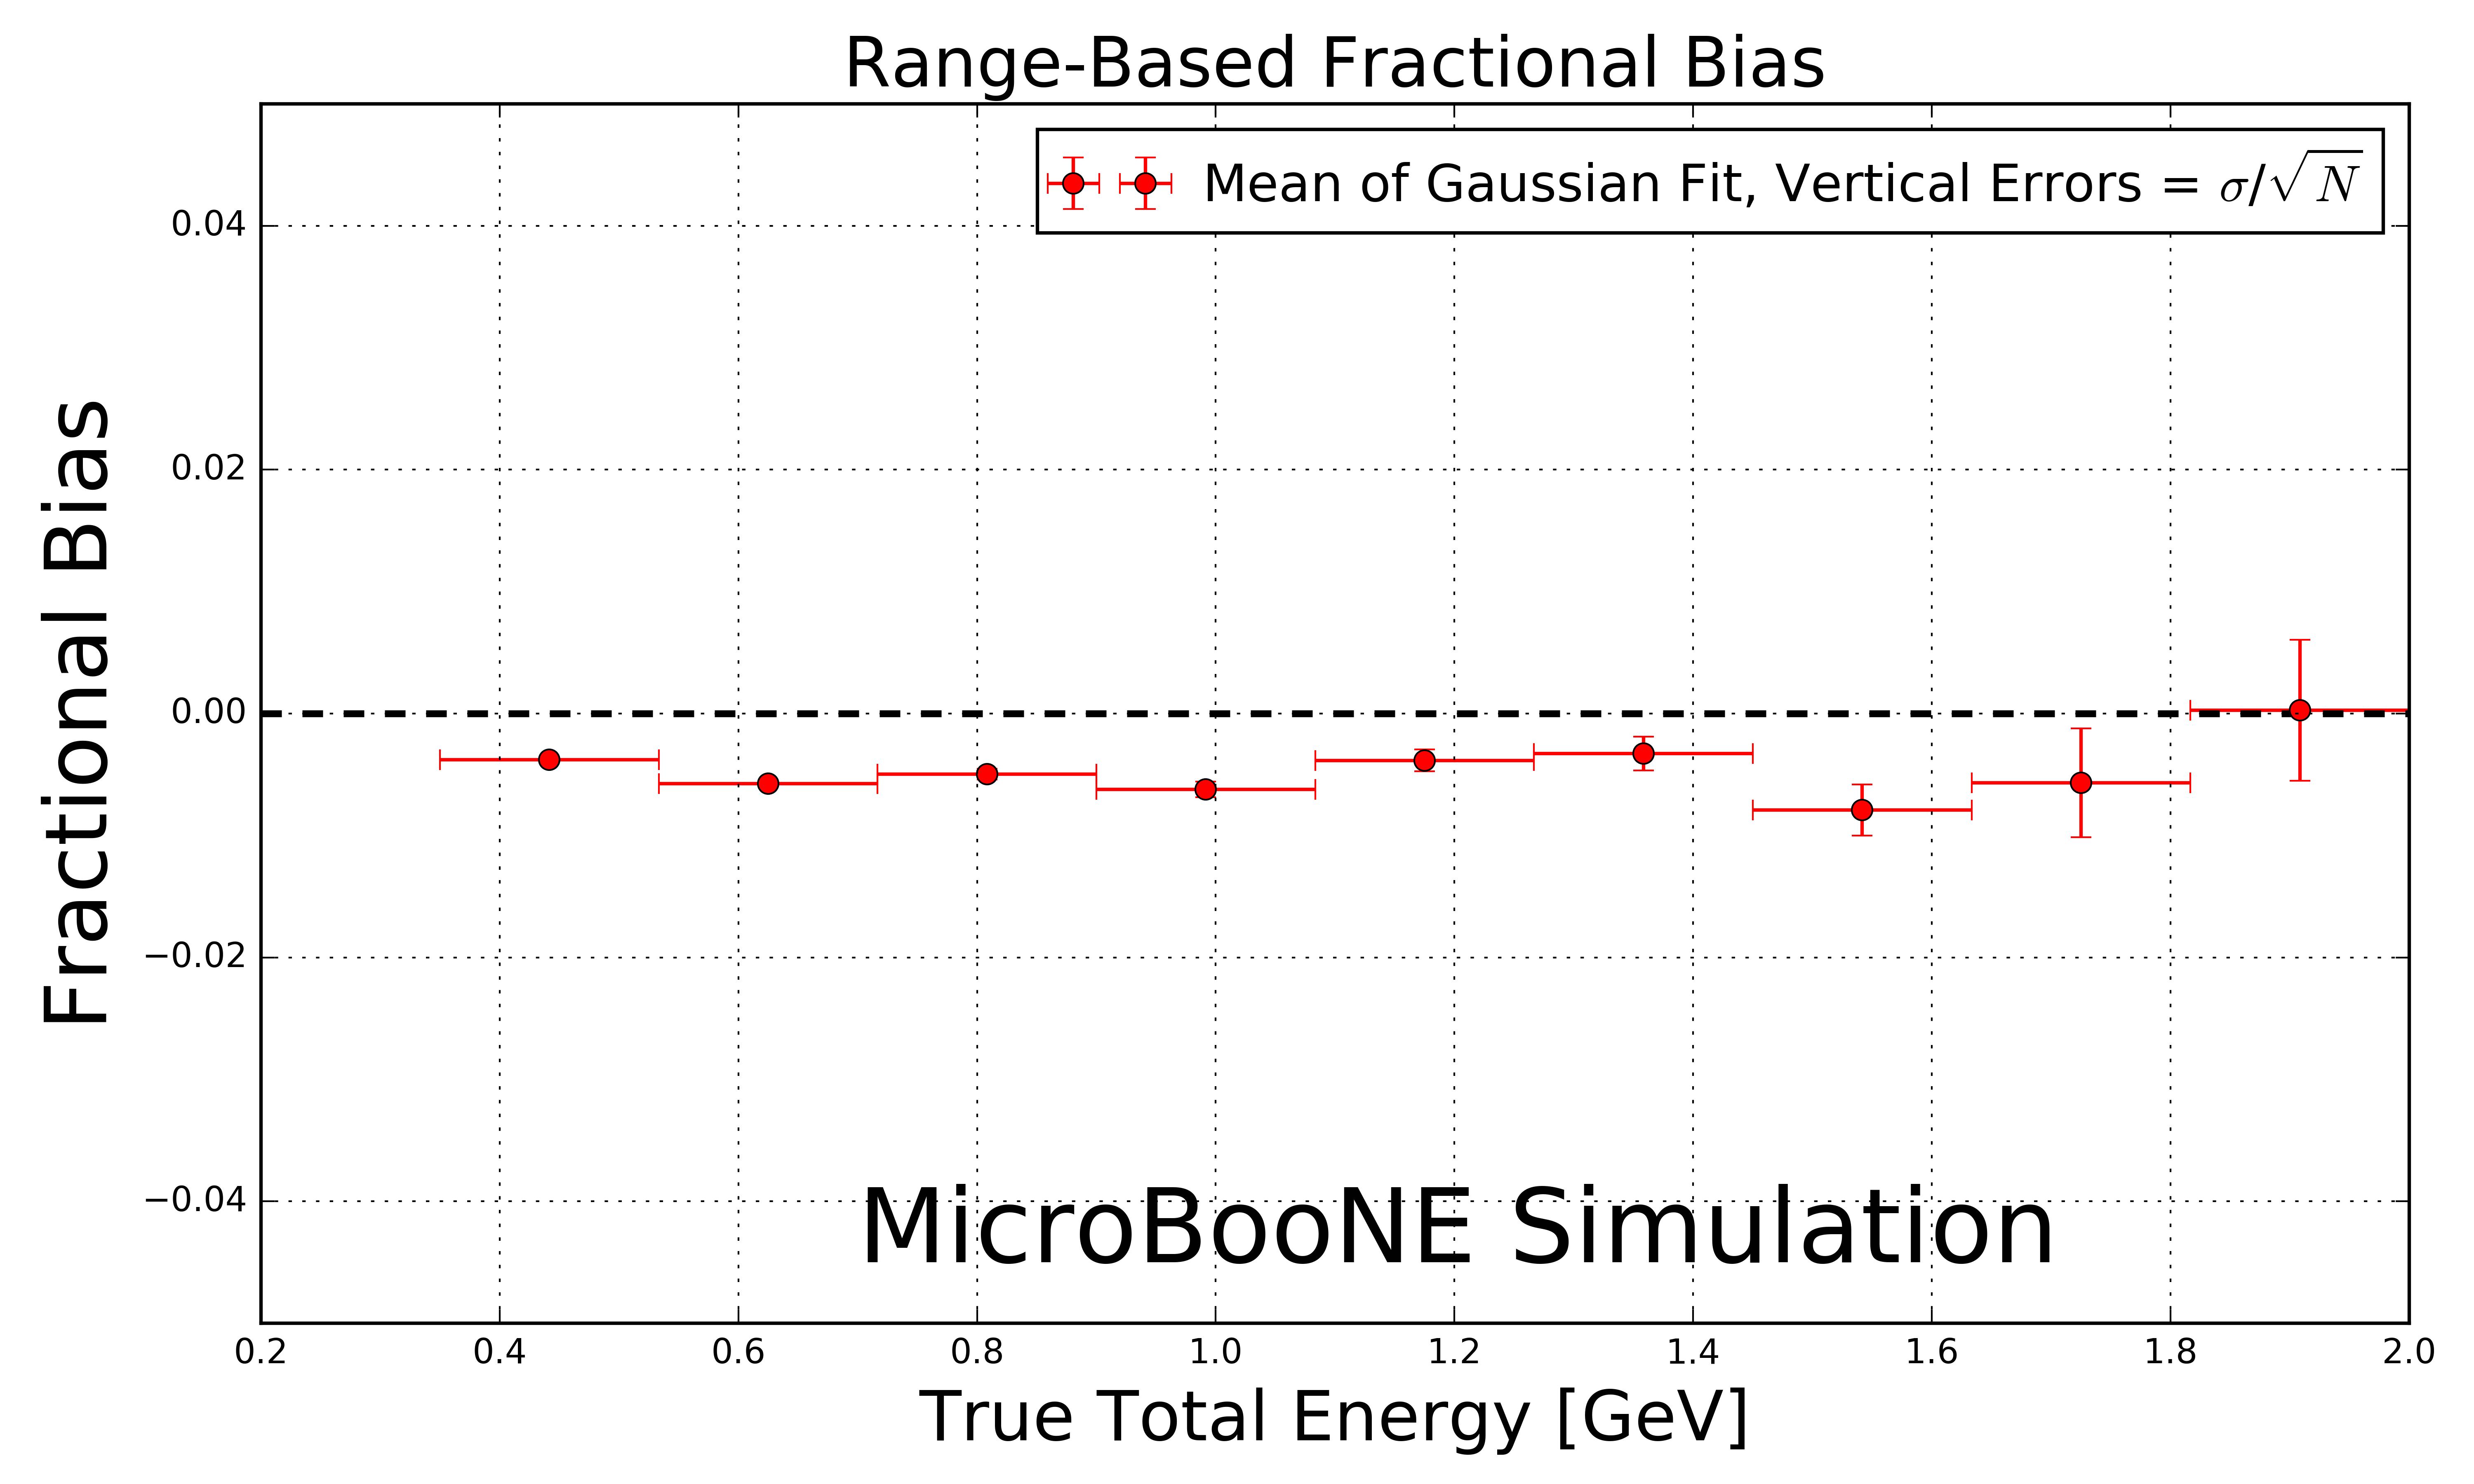
\includegraphics[width=0.7\textwidth]
	{Figures/true_range_bias_MCBNBMCTrack.png}
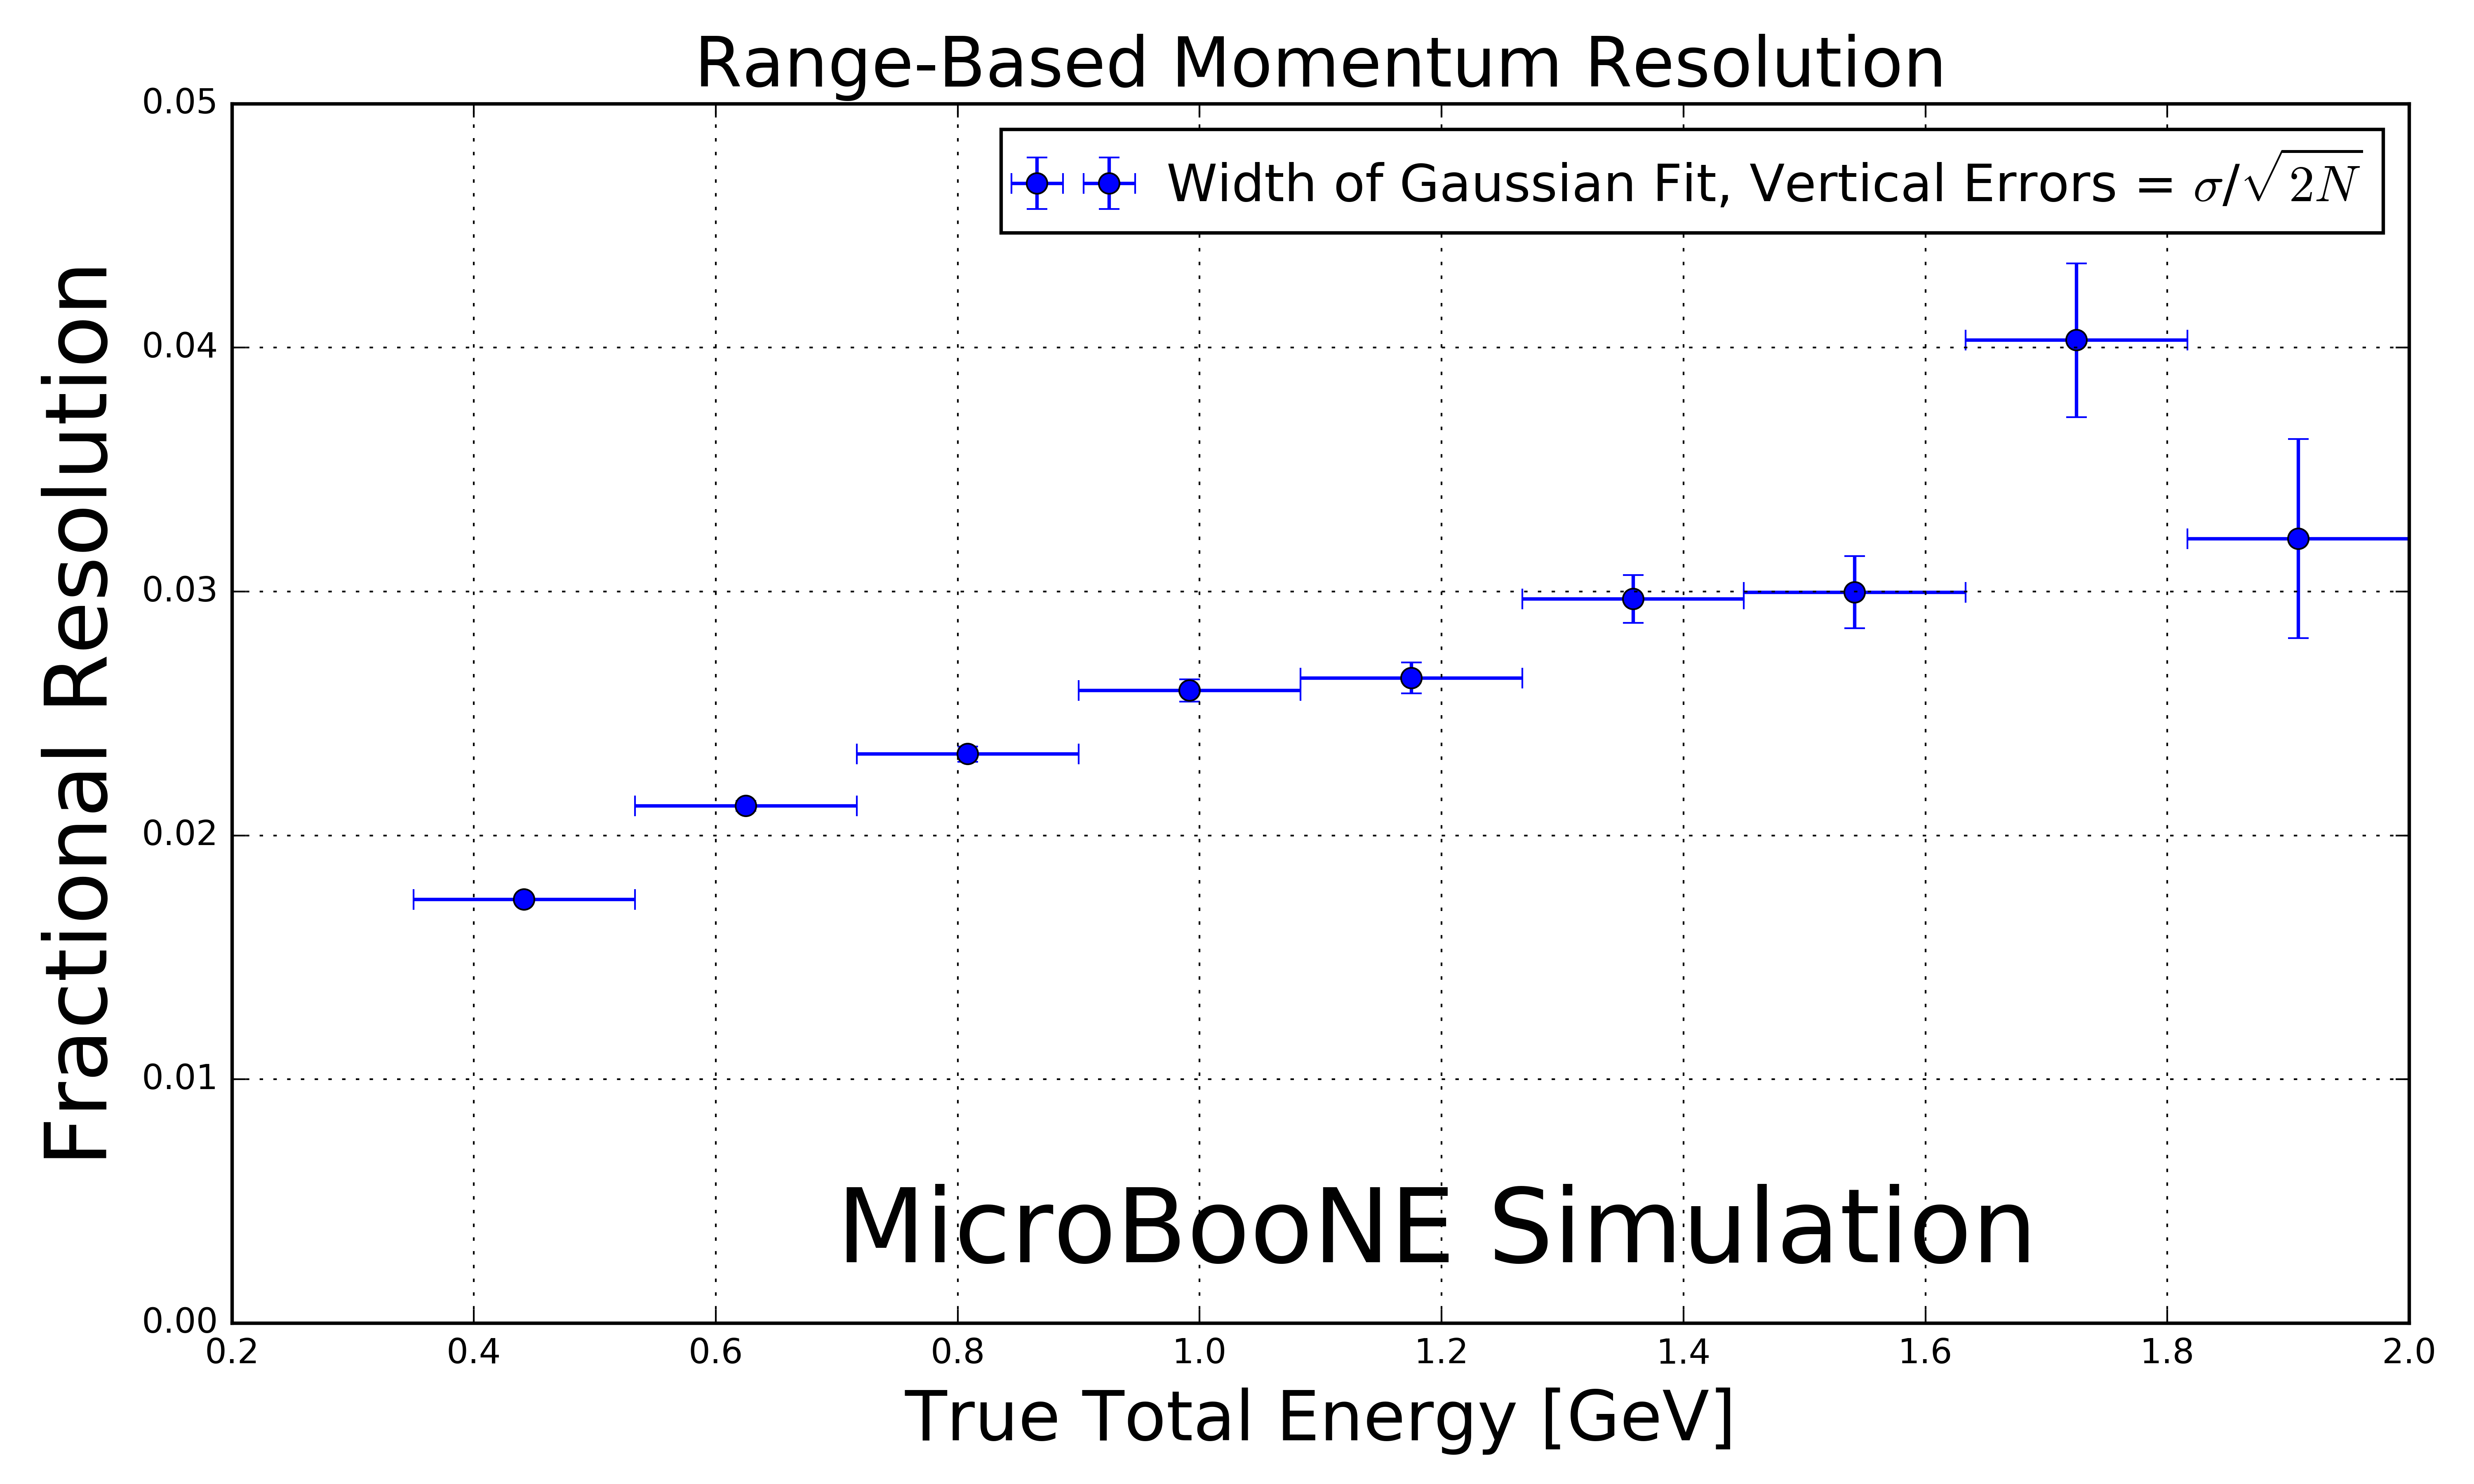
\includegraphics[width=0.7\textwidth]
	{Figures/true_range_resolution_MCBNBMCTrack.png}
\caption{\textit{Range-based energy fractional bias (top) and resolution (bottom) from a sample of simulated fully contained BNB neutrino-induced muons using true starting and stopping positions of the track. The bias is less than 1\% and the resolution is below $\approx$4\%.}}
\label{true_range_bias_resolution_MCTrack_fig}
\end{figure}






\section{MCS Performance on Beam Neutrino-Induced Muons in MicroBooNE Data}\label{data_performance_section}

\subsection{Input Sample}
The input sample to this portion of the analysis is $\sim$5e19 protons-on-target worth of triggered BNB neutrino interactions in MicroBooNE data, which is a small subset of the nominal amount of beam scheduled to be delivered to the detector. These events are run through a fully automated reconstruction chain which produces reconstructed objects including three-dimensional neutrino interaction points (vertices), three-dimensional tracks for each outgoing secondary particle from the interaction, and PMT-reconstructed optical flashes from the interaction scintillation light. The fiducial volume used in this analysis is defined as the full TPC volume reduced by 20 cm from both the cathode plane and the anode wire planes, by 26.5 cm from both the top and bottom walls of the TPC, by 20 cm from the beam-upstream wall of the TPC, and by 36.8 cm from the beam-downstream wall of the TPC.

\subsection{Event Selection}
The following selection cuts are placed on the aforementioned reconstructed objects to select $\nu_\mu$ charged-current interactions in which the muon track exiting the interaction vertex is fully contained within the fiducial volume:
\begin{enumerate}
\item The event must have at least one bright optical flash in coincidence with the expected BNB neutrino arrival time.
\item Two or more reconstructed tracks must originate from the same reconstructed vertex within the fiducial volume.
\item The span in $z-$ of the track must be within 70 cm of the $z-$ position of the optical flash as determined by the pulse height and timing of signals in the 32 PMTs.
\item For events with exactly two tracks originating from the vertex, additional calorimetric-based cuts are applied to mitigate backgrounds from in-time cosmics which produce Michel electrons that are reconstructed as a track.
\item The longest track originating from the vertex is assumed to be a muon, and it must be fully contained within the fiducial volume.
\item The longest track must be at least one meter long, in order to have enough sampling points in the MCS likelihood to obtain a reasonable estimate of its momentum.
\end{enumerate}

In this sample of MicroBooNE data, 598 events (tracks) remain after all event selection cuts. Each of these events (tracks) were scanned by hand with a 2D interactive event display showing the raw wire signals of the interaction from each wire plane, with the 2D projection of the reconstructed muon track and vertex overlaid. The scanning was done to ensure the track was well reconstructed with start point close to the reconstructed vertex and end point close to the end of the visible wire-signal track in all three planes. Additionally the scanning was to remove obvious mis-identification (MID) topologies such as cosmic rays inducing Michel electrons at the reconstructed neutrino vertex which were not successfully removed by the automated event selection cuts. After rejecting events (tracks) based on hand scanning, 396 tracks remain for analysis.


\subsection{Highland Validation}\label{highland_validation_section}
The Highland formula indicates that histogram of track segment-by-segment angular deviations in both the $x'$ and $y'$ directions divided by the width predicted from the Highland equation $\sigma_o^{HL}$ (Equation \ref{highland_eqtn}) should be gaussian with a width of unity. In order to calculate the momentum $p$ in the Highland equation, $p$ for each segment is computed with Equation \ref{segment_E_equation} where $E_t$ comes from the converged MCS computed momentum of the track. For each consecutive pair of segments in this sample of 396 tracks, the angular scatter in milliradians divided by the Highland expected RMS in millradians is an entry in the area-normalized histogram shown in Figure \ref{Highland_validation_fig}. From this figure we can see that the basis of the MCS technique is validated.

\begin{figure}[ht!]
\centering
	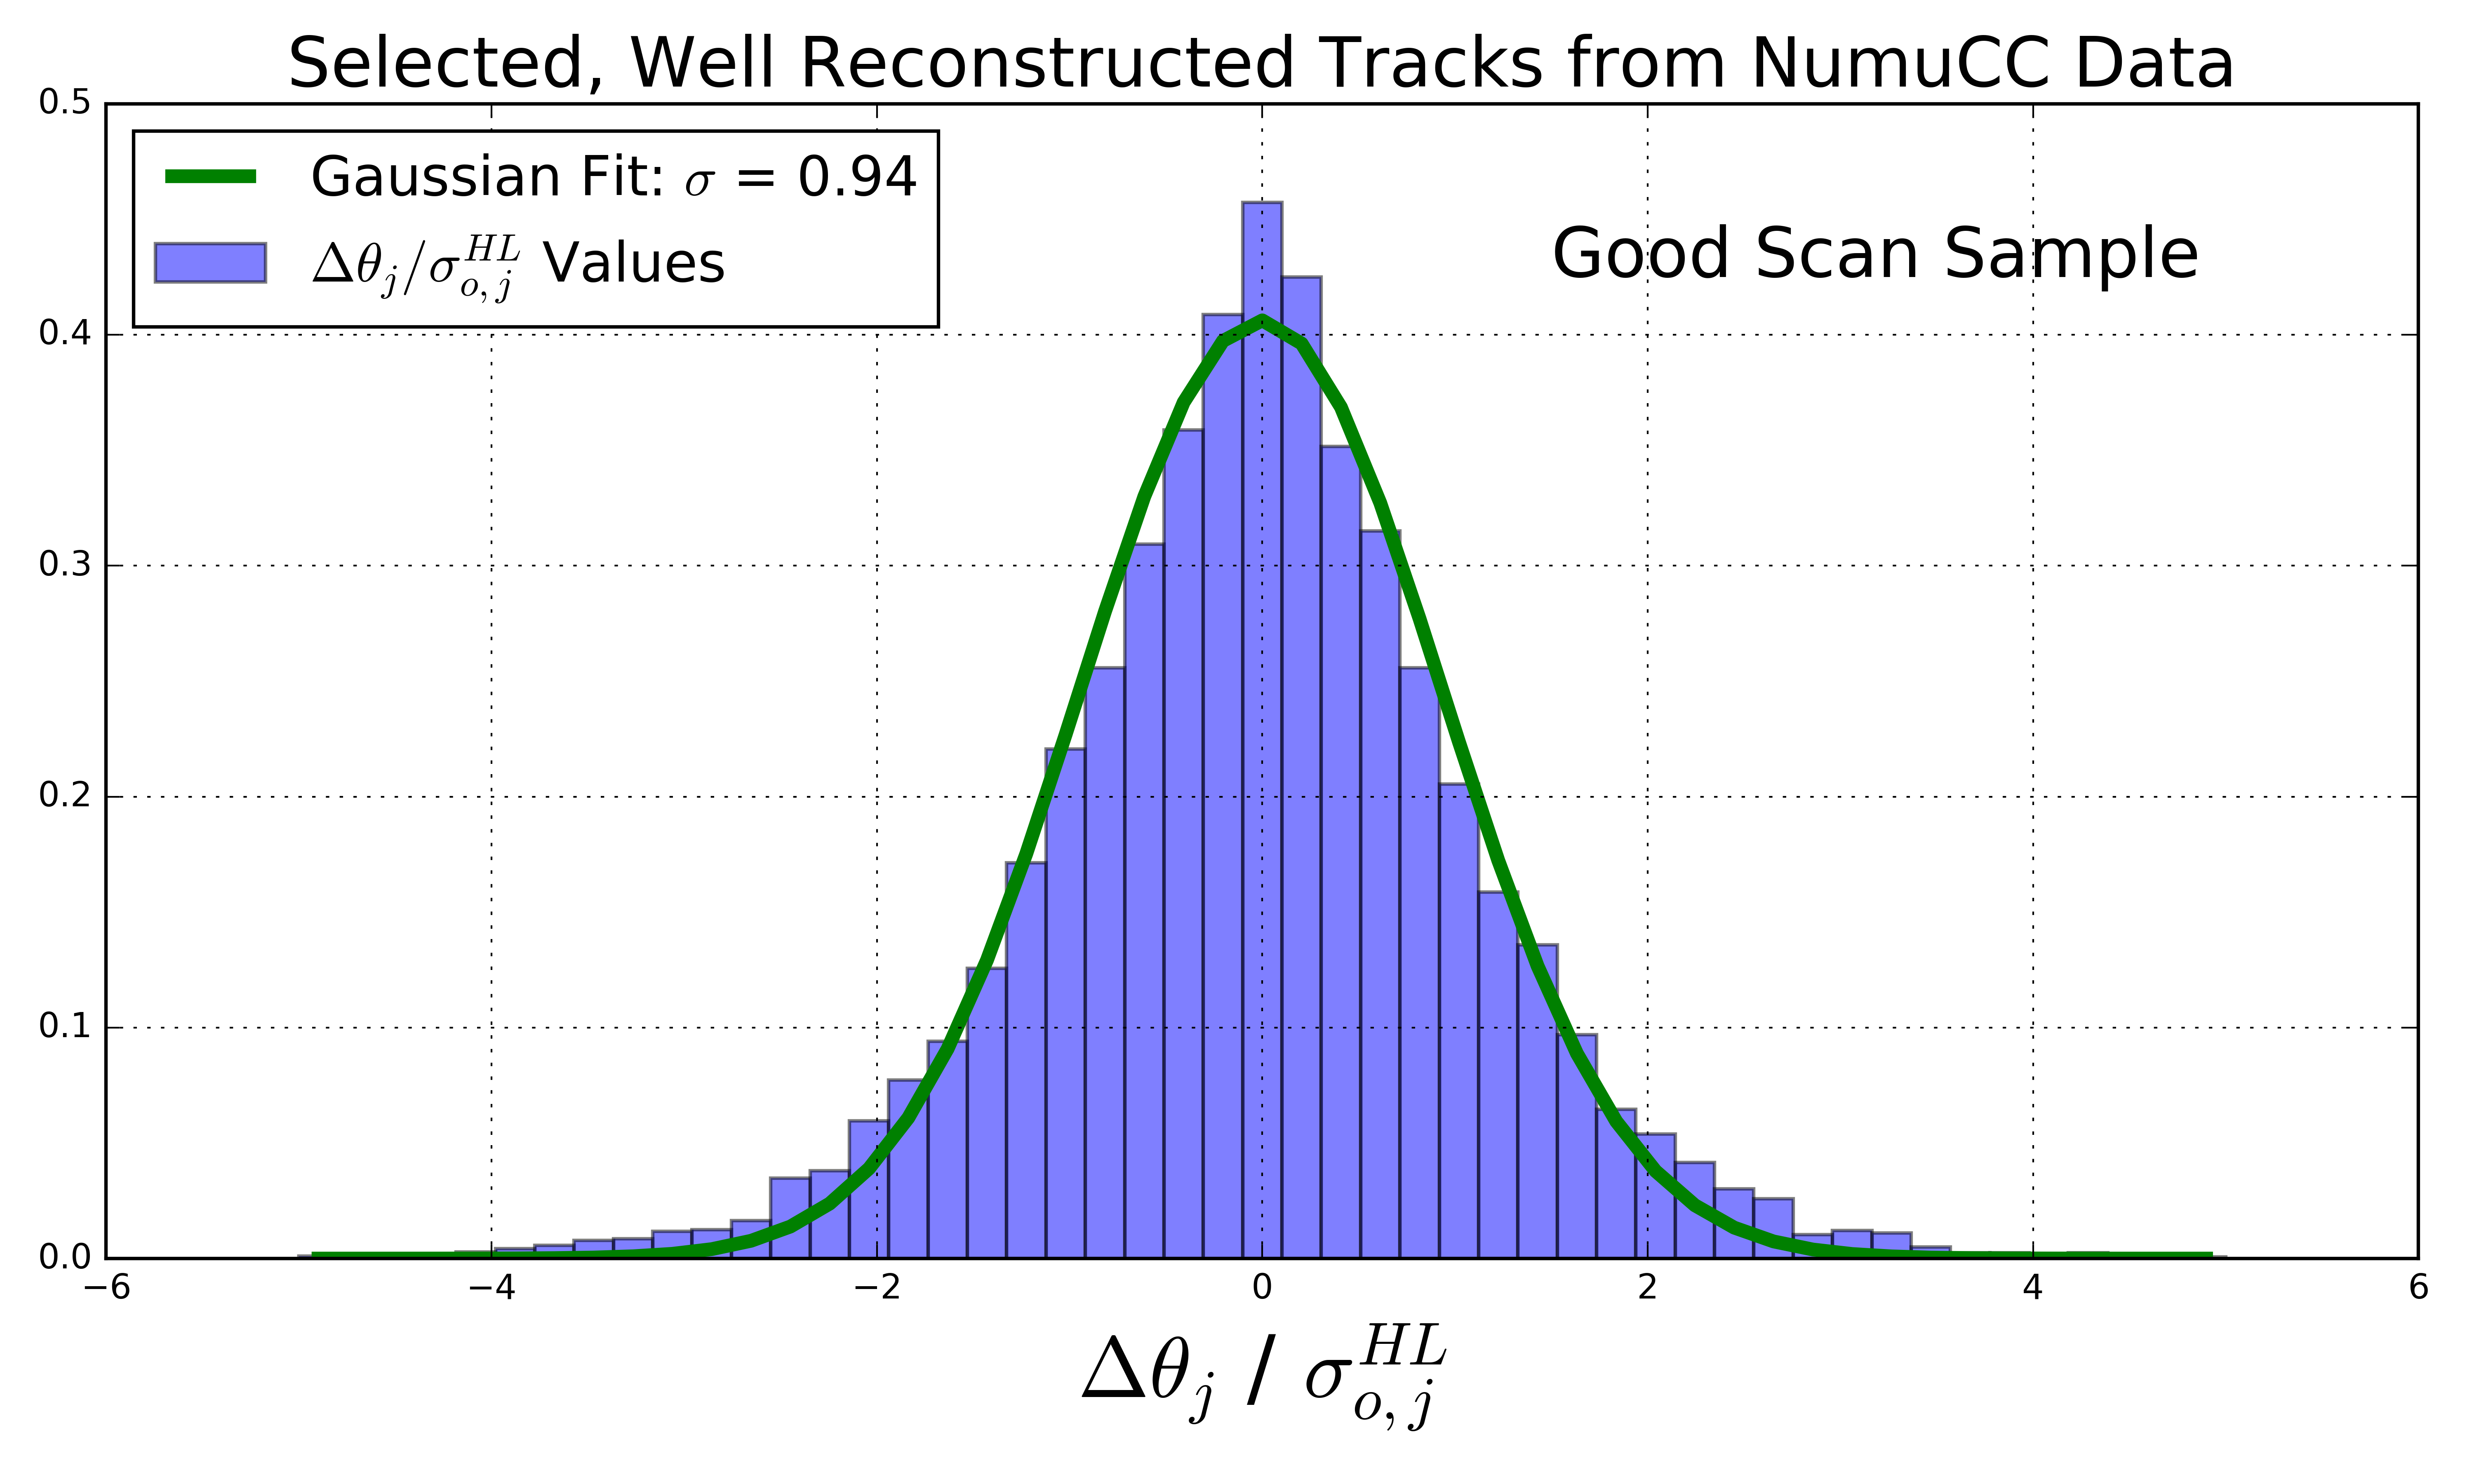
\includegraphics[width=0.7\textwidth]{Figures/Highland_validation_DataBNBSelectedRecoTrack_goodscan.png} \\
\caption{\textit{Segment-to-segment measured angular scatters in both the $x'$ and $y'$ directions divided by the Highland formula (Equation \ref{highland_eqtn}) predicted width $\sigma_o^{HL}$ for the automatically selected beam neutrino-induced fully contained muon sample in MicroBooNE data after hand scanning to remove poorly reconstructed tracks and obvious mis-identification (MID) topologies. A gaussian distribution with a width of unity indicates that the basis of the MCS technique is validated.}}\label{Highland_validation_fig}
\end{figure}


\subsection{MCS Momentum Validation}\label{MCS_Momentum_Validation_DataRecoTrack_section}

The MCS momentum versus range-based momentum for this sample of 396 tracks can be seen in Figure \ref{realdata_goodhandscan_fig}.

\begin{figure}[ht!]
\centering
	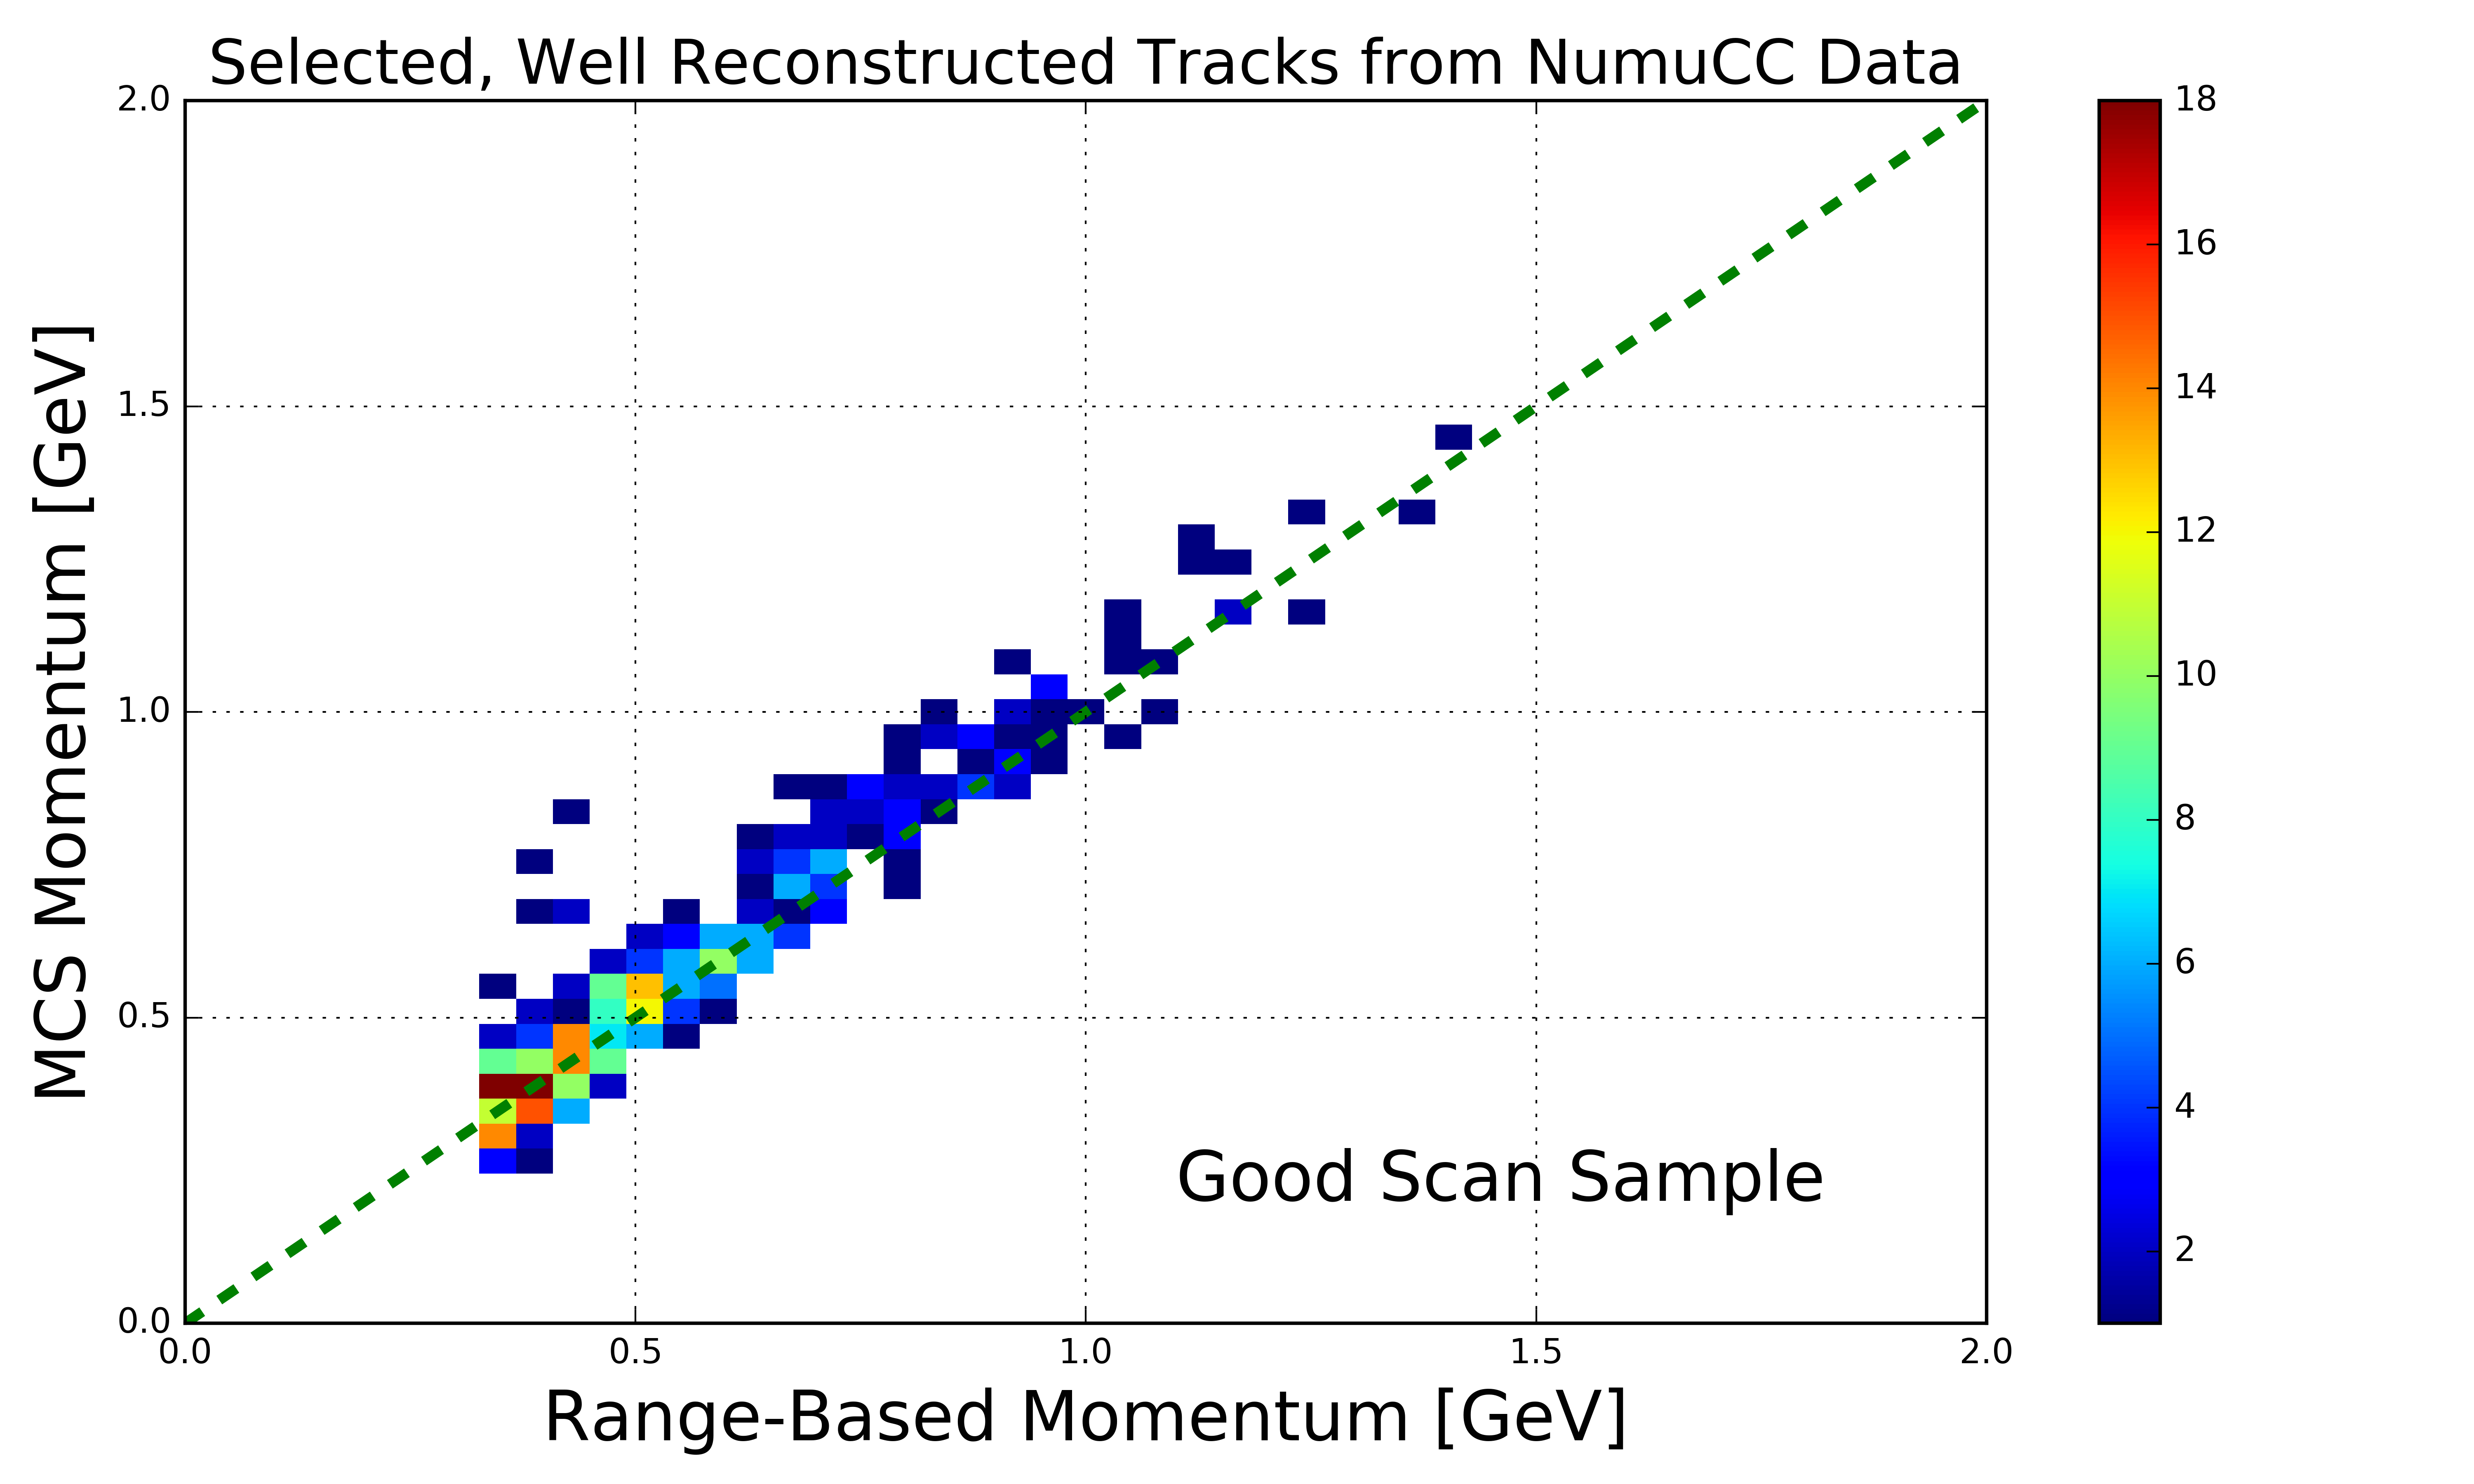
\includegraphics[width=0.7\textwidth]{Figures/MCS_range_momentum_DataRecoTracks_goodhandscan.png} \\
\caption{\textit{MCS computed momentum versus range momentum for the automatically selected beam neutrino-induced fully contained muon sample in MicroBooNE data after hand scanning to remove poorly reconstructed tracks and obvious mis-identification (MID) topologies.}}\label{realdata_goodhandscan_fig}
\end{figure}

% In order to compute a bias and a resolution, Figure \ref{MCS_range_momentum_MCTrack_fig} is sliced in bins of range momentum and a histogram of the fractional momentum difference ($\frac{p_{MCS}^{-1} - p_{range}^{-1}}{p_{range}^{-1}}$) is created for each bin\footnote{The choice of using inverse momentum is justified in Appendix \ref{inverse_p_justification_section}.}. This distribution is shown for three representative bins in Figure \ref{MCS_range_bias_resolution_MCTrack_slices_fig}, along with the gaussian fit to each.  The mean ($\mu$) of each gaussian fit is used to compute a bias as a function of range momentum, while the width ($\sigma$) of each distribution is used to compute a resolution. The bias and resolution for this momentum reconstruction method shown in Figure \ref{MCS_range_bias_resolution_MCTrack_fig}. This figure indicates a bias in the MCS momentum resolution on the order of a few percent, with a resolution that decreases from about 9\% for contained {\sc MCTracks} with true total momentum around 0.5 GeV (which corresponds to a length of about 1.7 meters) to below 3\% for contained {\sc MCTracks} with true total momentum greater than 0.8 GeV (which corresponds to a length of about 3.1 meters).





The MCS momentum fractional bias and resolution as a function of range-based momentum for this sample of 396 tracks is shown in Figure \ref{MCS_range_bias_resolution_DataRecoTrack_fig}. In order to compute this bias and resolution, distributions of fractional inverse momentum difference ($\frac{p_{MCS}^{-1} - p_{Range}^{-1}}{p_{Range}^{-1}}$) in bins of range-based momentum $p_{Range}$ are fit to gaussians and the mean of the fit determines the bias while the width of the fit determines the resolution for that bin. Inverse momentum is used here because the binned distributions are more gaussian, and therefore using the resulting fit parameters is more valid. Note that simply using the mean and RMS of the binned distributions yields similar results. Also shown in this figure are the bias and resolutions for an analogous simulated sample consisting of full BNB simulation with CORSIKA-generated\cite{corsika_ref} cosmic overlays passed through an identical reconstruction and event selection chain. Rather than hand scanning this sample, truth-based information was used by requiring the longest reconstructed track matched well in terms of true starting and stopping point of the $\nu_\mu$CC muon. These resolutions on the order of 10\% are consistent with the monte-carlo Kalman filter results presented by the ICARUS collaboration in this momentum range\cite{icarus_mcs_paper}.\\


\begin{figure}
\centering
	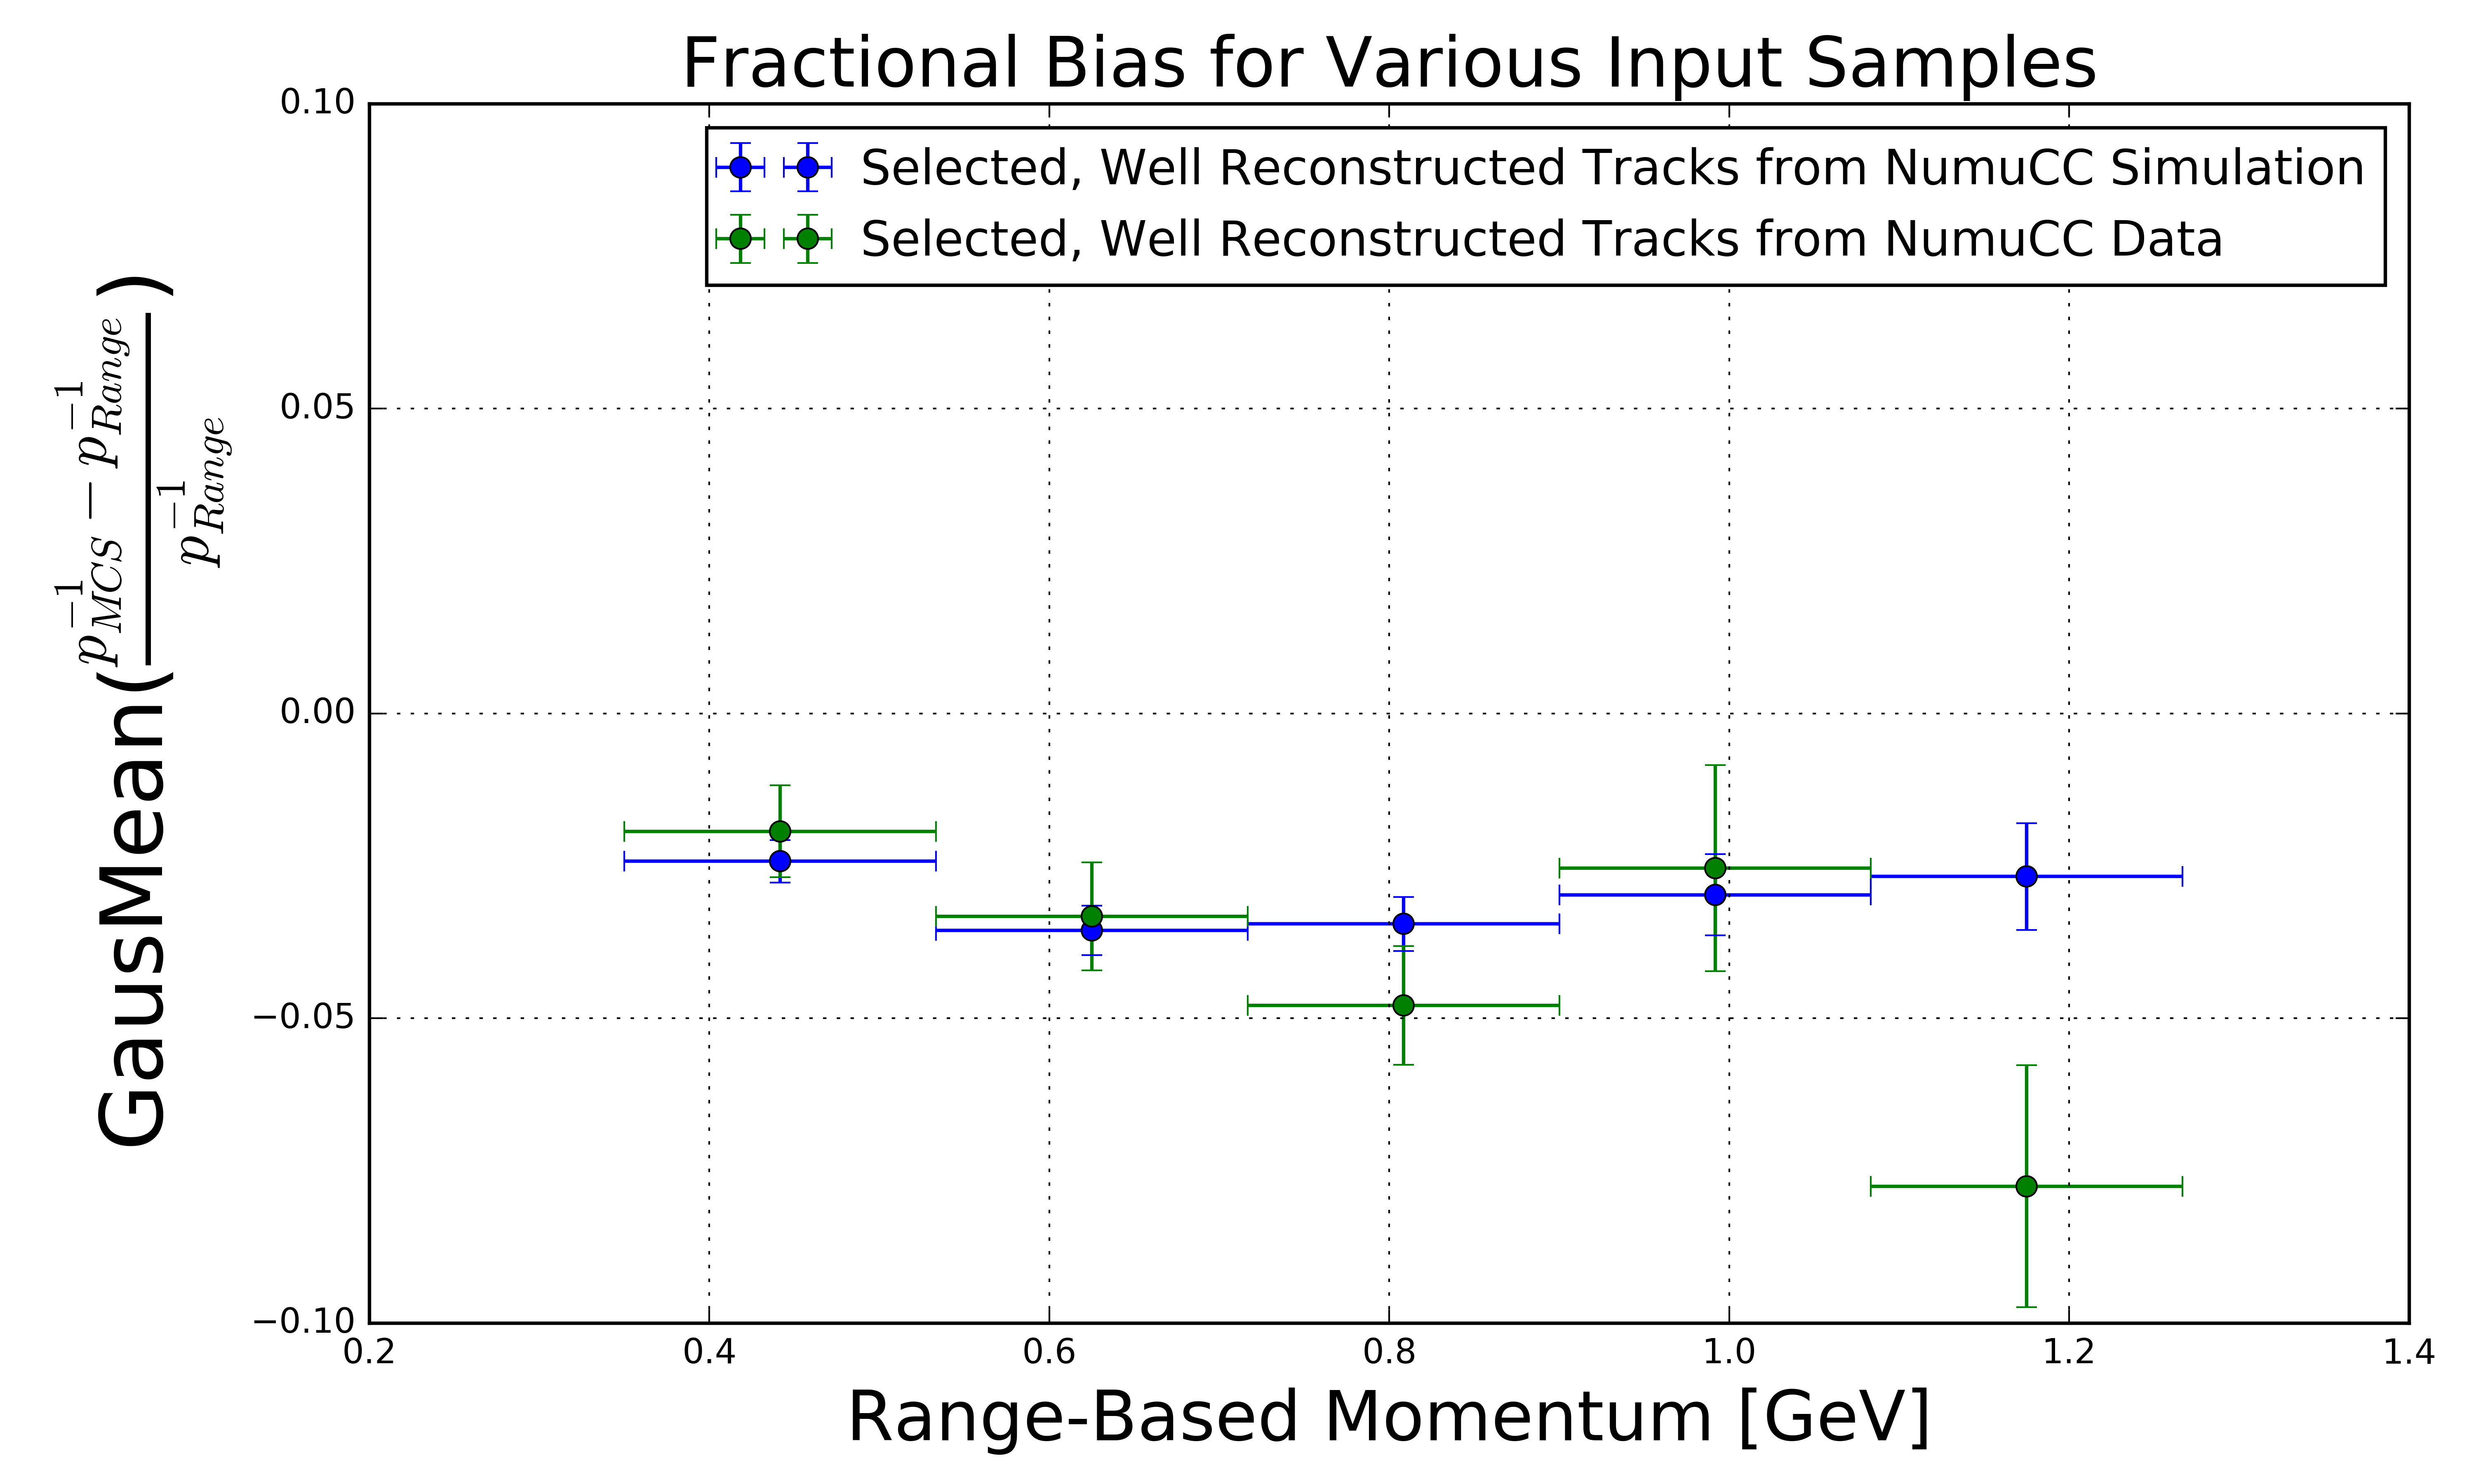
\includegraphics[width=0.7\textwidth]{Figures/MCS_range_bias_multiplesamples_publicplot.png}
	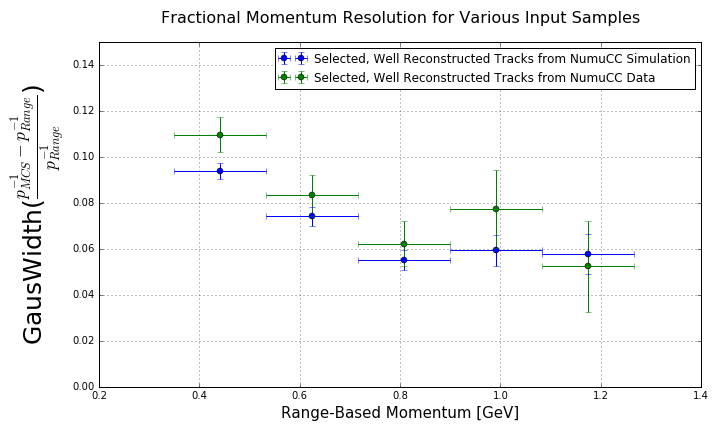
\includegraphics[width=0.7\textwidth]{Figures/MCS_range_resolution_multiplesamples_publicplot.png}
\caption{\textit{MCS momentum fractional bias (top) and resolution (bottom) for automatically selected contained $\nu_\mu$CC-induced muons from full simulated BNB events with cosmic overlay where the track matches with the true muon track (blue), and automatically selected contained $\nu_\mu$CC-induced muons from MicroBooNE data where the track is deemed well-reconstructed and likely-muon from hand scanning (green).}}\label{MCS_range_bias_resolution_DataRecoTrack_fig}
\end{figure}

This figure indicates a bias in the MCS momentum resolution on the order of a few percent, with a resolution that decreases from about 11\% (9\%) for contained reconstructed tracks in data (simulation) with range momentum around 0.45 GeV (which corresponds to a length of about 1.5 meters) to about 5\% (6\%) for contained reconstructed tracks in data (simulation) with range momentum about 1.15 GeV (which corresponds to a length of about 4.6 meters). In general bias and resolutions agree between data and simulation within uncertainty, with resolution slightly worse in data which can be attributed to the inefficiencies involved in hand scanning compared to the truth-based matching cut in simulation.











\section{Conclusions}
We have described the multiple coulomb scattering technique maximum likelihood method for estimating the momentum of a three dimensional reconstructed track in a LArTPC and have provided motivation for development of such a technique. This technique is a very valuable tool; it is the only way to estimate the momentum of an exiting muon and will be an important ingredient in future oscillation and cross-section measurements by MicroBooNE and within the LArTPC community as a whole. The performance of this method has been quantified both in simulation and in data on beam $\nu_\mu$CC-induced muons which are fully contained, with fractional bias less than 5\% and with fractional resolution below 12\%. 










% We suggest to always provide author, title and journal data:
% in short all the informations that clearly identify a document.

\begin{thebibliography}{99}

%These are sample bib items from the boilerplate template
% \bibitem{a}
% Author, \emph{Title}, \emph{J. Abbrev.} {\bf vol} (year) pg.

% \bibitem{b}
% Author, \emph{Title},
% arxiv:1234.5678.

% \bibitem{c}
% Author, \emph{Title},
% Publisher (year).

%1
  \bibitem{Aguilar-Arevalo:2013pmq} 
  A.~A.~Aguilar-Arevalo {\it et al.} 
  [MiniBooNE Collaboration],
  Improved Search for $\bar \nu_\mu \rightarrow \bar \nu_e$ Oscillations in the MiniBooNE Experiment,
  Phys.\ Rev.\ Lett.\  {\bf 110}, 161801 (2013).
  doi:10.1103/PhysRevLett.110.161801
  [arXiv:1207.4809 [hep-ex], arXiv:1303.2588 [hep-ex]].
  %%CITATION = doi:10.1103/PhysRevLett.110.161801;%%
  %384 citations counted in    

  \bibitem{ub_detectorpaper}
  R. Acciarri {\it et al.}
  [MicroBooNE Collaboration],
  Design and Construction of the MicroBooNE Detector,
  \url{http://microboone-docdb.fnal.gov:8080/cgi-bin/RetrieveFile?docid=5752&filename=MicroBooNE_DetectorPaper_Version4.0.pdf&version=3}

  %2
  \bibitem{lartpc}
  S. ~Lockwitz, 
  The MicroBooNE LArTPC,
  http://www-microboone.fnal.gov/talks/dpfMicroBooNELArTPC.pdf.

  %4
  \bibitem{highland}
  V. ~L. ~Highland, 
  Some Practical Remarks on Multiple Scattering, 
  Nucl.\ Instrum.\ Methods\ {\bf 129} (1975)
  104-120.
 
  \bibitem{icarus_mcs_paper}
  A.~Ankowski {\it et al.} [ICARUS Collaboration],
  ``Measurement of through-going particle momentum by means of multiple scattering with the ICARUS T600 TPC,''
  Eur.\ Phys.\ J.\ C {\bf 48}, 667 (2006)
  doi:10.1140/epjc/s10052-006-0051-3
  [hep-ex/0606006].
  %%CITATION = doi:10.1140/epjc/s10052-006-0051-3;%%
  %44 citations counted in INSPIRE as of 01 Dec 2016

  % %5
  % \bibitem{leonidas1}
  % L. ~Kalousis, 
  % Momentum measurement via Multiple Coulomb
  % Scattering with the MicroBooNE detector, 
  % MicroBooNE Doc-DB-3733.


  % %3
  % \bibitem{leonidas2}
  % L. ~Kalousis, 
  % Muon momentum measurement via Multiple Coulomb Scattering in argon,
  % MicroBooNE Doc-DB-4050.

 %7
  \bibitem{Marshall:2015rfa} 
  J.~S.~Marshall and M.~A.~Thomson,
  %``The Pandora Software Development Kit for Pattern Recognition,''
  Eur.\ Phys.\ J.\ C {\bf 75}, no. 9, 439 (2015)
  doi:10.1140/epjc/s10052-015-3659-3
  [arXiv:1506.05348 [physics.data-an]].

  %8
  \bibitem{MIPenergysource}
  D. E. Groom, N. V. Mokhov and S. Striganov, ``Muon Stopping Power and Range Tables: 10 MeV - 100 TeV'' Table 5,
  http://pdg.lbl.gov/2012/AtomicNuclearProperties/adndt.pdf


  %9
  \bibitem{PDG_spline_table} Table 289: Muons in Liquid argon (Ar) \url{http://pdg.lbl.gov/2012/AtomicNuclearProperties/MUON_ELOSS_TABLES/muonloss_289.pdf}


  \bibitem{corsika_ref} D. Heck, J. Knapp, J. N. Capdevielle, G. Schatz, T. Throw, \emph{CORSIKA: A Monte Carlo Code to Simulate Extensive Air Showers}, Forschungszentrum Karlsruhe Report FZKA 6019 (1998)

  % %6
  % \bibitem{CCIncInternalNote}
  % An et al,
  % Selection of charged-current $\nu_\mu$ inclusive events - Internal Note,
  % MicroBooNE Doc-DB-5851
  % \url{http://microboone-docdb.fnal.gov:8080/cgi-bin/RetrieveFile?docid=5851&filename=cc-incl-neutrino2016-v2.7.pdf&version=9}





% Please avoid comments such as "For a review'', "For some examples",
% "and references therein" or move them in the text. In general,
% please leave only references in the bibliography and move all
% accessory text in footnotes.

% Also, please have only one work for each \bibitem.


\end{thebibliography}
\end{document}




%%%%%%%%%%%%%%%%%%% ORIGINAL JINST BOILERPLATE CONTENT BELOW %%%%%%%%%%%%%%%%%%%%%%%%%%%%%%%
% For internal references use label-refs: see section~\ref{sec:intro}.
% Bibliographic citations can be done with cite: refs.~\cite{a,b,c}.
% When possible, align equations on the equal sign. The package
% \texttt{amsmath} is already loaded. See \eqref{eq:x}.
% \begin{equation}
% \label{eq:x}
% \begin{split}
% x &= 1 \,,
% \qquad
% y = 2 \,,
% \\
% z &= 3 \,.
% \end{split}
% \end{equation}
% Also, watch out for the punctuation at the end of the equations.


% If you want some equations without the tag (number), please use the available
% starred-environments. For example:
% \begin{equation*}
% x = 1
% \end{equation*}

% The amsmath package has many features. For example, you can use use
% \texttt{subequations} environment:
% \begin{subequations}\label{eq:y}
% \begin{align}
% \label{eq:y:1}
% a & = 1
% \\
% \label{eq:y:2}
% b & = 2
% \end{align}
% and it will continue to operate across the text also.
% \begin{equation}
% \label{eq:y:3}
% c = 3
% \end{equation}
% \end{subequations}
% The references will work as you'd expect: \eqref{eq:y:1},
% \eqref{eq:y:2} and \eqref{eq:y:3} are all part of \eqref{eq:y}.

% A similar solution is available for figures via the \texttt{subfigure}
% package (not loaded by default and not shown here).
% All figures and tables should be referenced in the text and should be
% placed on the page where they are first cited or in
% subsequent pages. Positioning them in the source file
% after the paragraph where you first reference them usually yield good
% results. See figure~\ref{fig:i} and table~\ref{tab:i}.

% \begin{figure}[htbp]
% \centering % \begin{center}/\end{center} takes some additional vertical space
% \includegraphics[width=.4\textwidth,trim=30 110 0 0,clip]{example-image-a}
% \qquad
% \includegraphics[width=.4\textwidth,origin=c,angle=180]{example-image-b}
% % "\includegraphics" from the "graphicx" permits to crop (trim+clip)
% % and rotate (angle) and image (and much more)
% \caption{\label{fig:i} Always give a caption.}
% \end{figure}


% \begin{table}[htbp]
% \centering
% \caption{\label{tab:i} We prefer to have borders around the tables.}
% \smallskip
% \begin{tabular}{|lr|c|}
% \hline
% x&y&x and y\\
% \hline
% a & b & a and b\\
% 1 & 2 & 1 and 2\\
% $\alpha$ & $\beta$ & $\alpha$ and $\beta$\\
% \hline
% \end{tabular}
% \end{table}

% We discourage the use of inline figures (wrapfigure), as they may be
% difficult to position if the page layout changes.

% We suggest not to abbreviate: ``section'', ``appendix'', ``figure''
% and ``table'', but ``eq.'' and ``ref.'' are welcome. Also, please do
% not use \texttt{\textbackslash emph} or \texttt{\textbackslash it} for
% latin abbreviaitons: i.e., et al., e.g., vs., etc.



% \section{Sections}
% \subsection{And subsequent}
% \subsubsection{Sub-sections}
% \paragraph{Up to paragraphs.} We find that having more levels usually
% reduces the clarity of the article. Also, we strongly discourage the
% use of non-numbered sections (e.g.~\texttt{\textbackslash
%   subsubsection*}).  Please also see the use of
% ``\texttt{\textbackslash texorpdfstring\{\}\{\}}'' to avoid warnings
% from the hyperref package when you have math in the section titles



% \appendix
% \section{Some title}
% Please always give a title also for appendices.





% \acknowledgments

% This is the most common positions for acknowledgments. A macro is
% available to maintain the same layout and spelling of the heading.

% \paragraph{Note added.} This is also a good position for notes added
% after the paper has been written.





